\mode<presentation>
{
  \usetheme{Boadilla}
}

\usepackage[utf8]{inputenc}
\usepackage{booktabs}

\usepackage{minted}
%\usepackage[draft]{minted}
\setminted{frame=single}

\title[Fuss-free data validation]{Fuss-free data validation without
  using exceptions}
\subtitle{Scala, Rust, Swift, Haskell}
\author{Franklin Chen \\ \url{http://franklinchen.com/}}
\institute{\href{http://www.codeandsupply.co/}{Pittsburgh Code and Supply}}
\date[April 9, 2015]{\href{http://www.meetup.com/Pittsburgh-Code-Supply/events/221130516/}{April 9, 2015}}

\subject{Talks}

%\AtBeginSection[]
%{
%  \begin{frame}<beamer>{Outline}
%    \tableofcontents[currentsection,subsectionstyle=hide]
%  \end{frame}
%}

\begin{document}

\maketitle

\begin{abstract}
The process of data validation can be messy and annoying, especially in the case of composite data where there could be many sources of errors and a need to collect all the errors found rather than bail out upon finding the first one. In practice, what often happens is that thorough validation ends up not being done because it's too painful to code. Martin Fowler recently wrote an article about the problem and proposed a solution \url{http://martinfowler.com/articles/replaceThrowWithNotification.html} but it is also painful.

There is a very clean solution that can be expressed in any language, so we will show the language-independent concepts so that you can use them anywhere.

However, since the solution is particularly concise to express in a certain class of languages that includes Scala, Rust, Swift, and Haskell, we will present concrete code in Scala, Rust, Swift, and Haskell to illustrate the concepts.
\end{abstract}

\begin{frame}
  \titlepage{}
\end{frame}

\section*{Outline}

\begin{frame}{Outline}
  \tableofcontents[subsectionstyle=hide]
\end{frame}

\section{Introduction}

\subsection{Goals}

\begin{frame}{Goals}
  \begin{itemize}
  \item Explain concepts using fully worked-out example
  \item Show real code (it's all up on GitHub)
  \item Hope you learn something you go out and \emph{use}
  \end{itemize}
\end{frame}

\subsection{Why cover four languages?}

\begin{frame}{Why cover four languages?}
  \begin{block}{Pittsburgh Code and Supply's polyglot advantage}
    \begin{itemize}
    \item Opportunity for you to explore a new language, and compare
      different designs
    \item More efficient than giving multiple presentation about the
      exact same concepts
    \end{itemize}
  \end{block}

  \begin{block}{Why Scala, Rust, Swift, Haskell?}
    \begin{itemize}
    \item First-class functions
    \item Tagged union types
    \end{itemize}
  \end{block}

  But any language with first-class functions can be used:
  \begin{itemize}
  \item JavaScript, etc.
  \end{itemize}

  \begin{alertblock}{Swift is still changing}
    Limited Swift code examples: language and compiler
    not stable (Swift 1.2 was officially released \emph{yesterday}\ !)
  \end{alertblock}
\end{frame}


\section{A data validation example task}

\begin{frame}{A data validation example task}
  From Martin Fowler's article, \href{http://martinfowler.com/articles/replaceThrowWithNotification.html}{``Replacing Throwing Exceptions with Notification in Validations''}:
  \begin{itemize}
  \item Goal: create a valid event from a theater booking request
  \item Given: a date string that is possible null, a number of seats
    that is possible null
  \item Validate:
    \begin{itemize}
    \item Possibly null date string
      \begin{itemize}
      \item Date string must not be null
      \item Date string must actually parse to a date
      \item Request date must not be earlier than now
      \end{itemize}
    \item Possibly null number of seats
      \begin{itemize}
      \item Number of seats must not be null
      \item Number of seats must be positive
      \end{itemize}
    \end{itemize}
  \end{itemize}

\end{frame}

\begin{frame}{Java code}
  \inputminted{java}{BookingRequest.java}
\end{frame}

\section{Models of computation}

\subsection{Normal execution}

\begin{frame}{Normal execution}
  \begin{itemize}
  \item A thread of execution, toward a destination
  \item Stack of pending operations
  \item When an operation is complete, pops off the stack
  \end{itemize}
\end{frame}

\subsection{Exceptions}

\begin{frame}{Exceptions considered problematic}
  \begin{alertblock}{Exceptions mean jumping up the stack}
    \begin{itemize}
    \item Have to explicitly watch for and catch them
    \item Tedious to collect more than one error if exceptions are
      used
    \item What happens when there is concurrency?
    \end{itemize}
  \end{alertblock}

  \begin{block}{Some languages don't have exceptions}
    \begin{itemize}
    \item C
    \item Go
    \item Rust
    \item Swift
    \end{itemize}
  \end{block}
\end{frame}

\subsection{Railway-oriented programming}

\begin{frame}{Railway-oriented programming}
  \href{http://fsharpforfunandprofit.com/posts/recipe-part2/}{Railway-oriented
    programming}:
  \begin{itemize}
  \item Keeping computation on the tracks.
  \item Cleanly handle track-switching and merging.
  \end{itemize}
\end{frame}

\subsection{The unloved second track in many languages}

\begin{frame}{\mintinline{scala}{null}: the unloved second track}
  \begin{itemize}
  \item \mintinline{scala}{null} is
    \href{http://www.infoq.com/presentations/Null-References-The-Billion-Dollar-Mistake-Tony-Hoare}{Tony Hoare's billion-dollar mistake}, invented in 1965
  \item Adds a second track to every single computation involving a
    reference type
  \item Null Pointer Exceptions, seg faults
  \end{itemize}

  No more mention of \mintinline{scala}{null} here!
  \begin{itemize}
  \item All four languages mentioned have an improvement we take as a
    starting point.
  \end{itemize}
\end{frame}

\section{\mintinline{scala}{Option[T]}}

\subsection{Definition}

\begin{frame}{\mintinline{scala}{Option[T]}}
  \begin{table}
    \begin{tabular}{| l | l | l | l | l |}
      \toprule
      & Scala & Rust & Swift & Haskell \\
      \midrule
      Type & \href{http://www.scala-lang.org/api/current/index.html\#scala.Option}{\mintinline{scala}{Option[T]}} &
        \href{http://doc.rust-lang.org/1.0.0-beta/std/option/enum.Option.html}{\mintinline{rust}{Option<T>}} &
        \href{https://developer.apple.com/library/ios/documentation/Swift/Conceptual/Swift_Programming_Language/Types.html\#//apple_ref/doc/uid/TP40014097-CH31-ID452}{\mintinline{swift}{Optional<T>}}\footnote{Abbreviated \mintinline{swift}{T?}} &
        \href{http://hackage.haskell.org/package/base-4.8.0.0/docs/Data-Maybe.html}{\mintinline{haskell}{Maybe t}} \\
      \midrule
      Nonexistence & \mintinline{scala}{None} &
        \mintinline{rust}{None} &
        \mintinline{swift}{.None}\footnote{Abbreviated \mintinline{swift}{nil}} &
        \mintinline{haskell}{Nothing} \\
      Existence & \mintinline{scala}{Some(x)} &
        \mintinline{rust}{Some(x)} &
        \mintinline{swift}{.Some(x)}\footnote{Special syntactic sugar available} &
        \mintinline{haskell}{Just x} \\
      \bottomrule
    \end{tabular}
  \end{table}
\end{frame}

\subsection{Chaining computations over \mintinline{scala}{Option[T]}}

\begin{frame}{Chaining computations over \mintinline{scala}{Option[T]}}
  \begin{figure}
    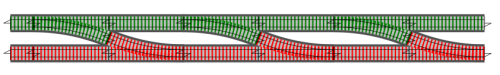
\includegraphics[width=\textwidth]{Recipe_RailwaySwitch3.png}
  \end{figure}
  \begin{example}{Railway chaining values of an \mintinline{scala}{Option} type}
    \begin{itemize}
    \item If encountering a \mintinline{scala}{None}:
      \begin{itemize}
      \item Bail out permanently to the failure track
      \end{itemize}
    \item Else if encountering a \mintinline{scala}{Some(x)}:
      \begin{itemize}
      \item Stay on the success track
      \end{itemize}
    \end{itemize}
  \end{example}
\end{frame}

\begin{frame}{Scala: chaining syntactic sugar for \mintinline{scala}{Option[T]}}
  \begin{example}{``Find the winner: your best friend's oldest sister's
      youngest child''}
    \inputminted{scala}{OptionWinner.scala}
  \end{example}

  \begin{itemize}
  \item Scala's ``\mintinline{haskell}{for} comprehensions'' inspired by Haskell
  \item Generic for railway-oriented programming
  \end{itemize}
\end{frame}

\begin{frame}{Scala: non-sugar chaining for \mintinline{scala}{Option[T]}}
  \begin{example}{``Find the winner: your best friend's oldest sister's
      youngest child''}
    \inputminted{scala}{NoSugarOptionWinner.scala}
  \end{example}

  \begin{itemize}
  \item Sugar is preprocessed to this code \emph{before compilation}
  \end{itemize}
\end{frame}

\begin{frame}{Swift: chaining syntactic sugar for \mintinline{swift}{T?}}
  \begin{example}{``Find the winner: your best friend's oldest sister's
      youngest child''}
    \inputminted{swift}{OptionWinner.swift}
  \end{example}

  \begin{itemize}
  \item Swift's \href{https://developer.apple.com/library/ios/documentation/Swift/Conceptual/Swift_Programming_Language/OptionalChaining.html}{special
    chaining sugar}
  \item Specific to \mintinline{swift}{Optional} only!
  \end{itemize}
\end{frame}

\begin{frame}{Rust: no syntactic sugar for \mintinline{rust}{Option<T>}}
  \begin{example}{``Find the winner: your best friend's oldest sister's
      youngest child''}
    \inputminted{rust}{option_winner.rs}
  \end{example}

  \begin{itemize}
  \item Rust: no syntactic sugar
  \item
    \href{http://aturon.github.io/errors/signaling.html}{Deprecate}
    use of \mintinline{rust}{Option} for error signaling!
  \item Sugar provided for what Rust recommends instead (next topic)
  \end{itemize}
\end{frame}

\begin{frame}{Haskell: chaining syntactic sugar for \mintinline{haskell}{Maybe t}}
  \begin{example}{``Find the winner: your best friend's oldest sister's
      youngest child''}
    \inputminted{haskell}{OptionWinner.hs}
  \end{example}

  \begin{itemize}
  \item Haskell's ``\mintinline{haskell}{do} notation'' invented in 1993
  \end{itemize}
\end{frame}

\subsection{\mintinline{scala}{Option} considered harmful}

\begin{frame}{\mintinline{scala}{Option} considered harmful}
  \begin{alertblock}{Warning}
    An \mintinline{scala}{Option}-chained failure gives \emph{zero information} about
    \emph{why} and \emph{where} something failed!
  \end{alertblock}

  When \mintinline{scala}{winner(person)} returns
  \mintinline{scala}{None}:
  \begin{itemize}
  \item Did the person's best friend's oldest sister not have any children?
  \item Or did the person's best friend not have any sisters?
  \item Or did the person not have any friends?
  \end{itemize}

  \begin{alertblock}{Knowledge is power}
    ``Enquiring minds want to know!''
  \end{alertblock}
\end{frame}

\section{\mintinline{scala}{Either[E, T]}}

\subsection{Definition}

\mintinline{scala}{Either[E, T]} generalizes \mintinline{scala}{Option[T]}:
\begin{itemize}
\item Success remains the same
\item Failure is no longer \mintinline{scala}{None}, but is a value of some error
  type \mintinline{scala}{E} you choose
\end{itemize}

\begin{frame}{\mintinline{scala}{Either[E, T]}}
  \begin{table}
    \begin{tabular}{| l | l | l | l |}
      \toprule
      & Scala & Swift & Haskell \\
      \midrule
      Type &
             \href{http://www.scala-lang.org/api/current/index.html\#scala.Either}{\mintinline{scala}{Either[E, T]}}\footnote{The \href{https://github.com/scalaz/scalaz}{Scalaz} library provides an improved version called \mintinline{scala}{E \/ T} we will prefer} &
        \href{https://github.com/typelift/Swiftx/blob/master/Swiftx/Either.swift}{\mintinline{swift}{Either<E, T>}}\footnote{\mintinline{swift}{Either<E, T>} \emph{not} in Swift's standard library, but provided in \href{https://github.com/typelift/Swiftx}{Swiftx}} &
        \href{http://hackage.haskell.org/package/base-4.8.0.0/docs/Data-Either.html}{\mintinline{haskell}{Either e t}} \\
      \midrule
      Bad & \mintinline{scala}{Left(e)} &
        \mintinline{swift}{.Left(e)} &
        \mintinline{haskell}{Left e} \\
      Good & \mintinline{scala}{Right(x)} &
        \mintinline{swift}{.Right(x)} &
        \mintinline{haskell}{Just x} \\
      \bottomrule
    \end{tabular}
  \end{table}

  \begin{table}
    \begin{tabular}{| l | l |}
      \toprule
      & Rust \\
      \midrule
      Type &
        \href{http://doc.rust-lang.org/1.0.0-beta/std/result/enum.Result.html}{\mintinline{rust}{Result<T, E>}}\footnote{Rust chose a more informative name, and placed success type param \mintinline{rust}{T} first} \\
      \midrule
      Bad & \mintinline{rust}{Err(e)} \\
      Good & \mintinline{rust}{Ok(x)} \\
      \bottomrule
    \end{tabular}
  \end{table}

\end{frame}

\begin{frame}{Converting between \mintinline{scala}{Option[T]} to
    \mintinline{scala}{E \/ T}}
  \begin{block}{Conversion is simple}
    Examples using Scalaz:


    \begin{description}
    \item[\mintinline{scala}{E \/ T} to \mintinline{scala}{Option}]
      ``Forget'' an error by replacing it with \mintinline{scala}{None}:
      \mint{scala}{optX = eitherX.toOption}
    \item[\mintinline{scala}{Option[T]} to \mintinline{scala}{E \/ T}]
      ``Add'' an error by replacing \mintinline{scala}{None} with an error:
      \mint{scala}{eitherX = optX.toRightDisjunction("some error")}
    \end{description}
  \end{block}
\end{frame}

\subsection{Chaining computations over \mintinline{scala}{Either[E, T]}}

\begin{frame}{Chaining computations over \mintinline{scala}{Either[E, T]}}
  \begin{figure}
    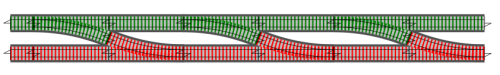
\includegraphics[width=\textwidth]{Recipe_RailwaySwitch3.png}
  \end{figure}

  Exact same concept as with \mintinline{scala}{Option[T]}.
\end{frame}

\begin{frame}{Scala: chaining syntactic sugar for \mintinline{scala}{E \/ T}}
  \begin{example}{``Find the winner: your best friend's oldest sister's
      youngest child''}
    \inputminted{scala}{ResultWinner.scala}
  \end{example}

  \begin{itemize}
  \item Exact same code as with \mintinline{scala}{Option[T]}!
  \item We are using Scalaz library's \href{https://github.com/scalaz/scalaz/blob/series/7.1.x/core/src/main/scala/scalaz/Either.scala}{disjunction} {\mintinline{scala}{E \/ T}}
    because standard Scala's \mintinline{scala}{Either[E, T]} has limitations
  \item Genericity of railway-oriented code: large topic in itself
  \end{itemize}
\end{frame}

\begin{frame}{Swift: no syntactic sugar for \mintinline{swift}{Either<E, T>}}
  \begin{example}{``Find the winner: your best friend's oldest sister's
      youngest child''}
    \inputminted{swift}{ResultWinner.swift}
  \end{example}

  \begin{itemize}
  \item Use
    \href{https://github.com/typelift/Swiftx}{Swiftx} library
    \item Swift does \emph{not} have general railway-oriented syntactic sugar
  \end{itemize}
\end{frame}

\begin{frame}{Rust: chaining syntactic sugar for \mintinline{rust}{Result<T, E>}}
  \begin{example}{``Find the winner: your best friend's oldest sister's
      youngest child''}
    \inputminted{rust}{result_winner.rs}
  \end{example}

  Rust
  \begin{itemize}
  \item Can use exactly the same non-sugar code as for
    \mintinline{rust}{Option<T>} if wanted
  \item Standard library has macro \mintinline{rust}{try!} for use with \mintinline{rust}{Result<T, E>}
  \item \emph{Does not have exceptions}, so ease of use of
    \mintinline{rust}{Result<T, E>} is critical!
  \end{itemize}
\end{frame}

\begin{frame}{Haskell: chaining syntactic sugar for \mintinline{haskell}{Either e t}}
  \begin{example}{``Find the winner: your best friend's oldest sister's
      youngest child''}
    \inputminted{haskell}{ResultWinner.hs}
  \end{example}

  \begin{itemize}
  \item Exact same code as with \mintinline{haskell}{Maybe t}!
  \end{itemize}
\end{frame}

% Do we need this?
%\subsection{How is \mintinline{scala}{Either} better than exceptions?}

\subsection{Constructors considered harmful}

\begin{frame}{Constructors considered harmful}
  \begin{itemize}
  \item Constructors in many languages do not return a result, so failures
    are indicated by either:
    \begin{itemize}
    \item Throwing an exception
    \item Return \mintinline{scala}{null} and setting an error object elsewhere
    \end{itemize}
  \item Alternative: ``factory method'' that returns an
    \mintinline{scala}{Either[SomeError, ThingToCreate]}
  \end{itemize}
\end{frame}

\begin{frame}{Constructing Seat: Scala}
  \inputminted{scala}{Seats.scala}
\end{frame}

\begin{frame}{Notes on clean module design}
  \begin{itemize}
  \item The constructor for \mintinline{scala}{Seats}:
    \begin{itemize}
    \item Is trivial, not
      \href{http://www.daedtech.com/beware-the-bloated-constructor}{bloated}:
      just saves off parameters into fields
    \item Is private, to guarantee only approved factory methods can call it
    \end{itemize}
  \item Errors:
    \begin{itemize}
    \item Each module defines its own set of errors as a union type,
      here called \mintinline{scala}{Error}
    \item (Here only one, \mintinline{scala}{BadCount})
    \end{itemize}
  \item Factory methods:
    \begin{itemize}
    \item Each \mintinline{scala}{Seats} factory method returns \mintinline{scala}{Error \/ Seats}
    \end{itemize}
  \end{itemize}
\end{frame}

\begin{frame}{Constructing Seat: Rust}
  \inputminted{rust}{seats.rs}
\end{frame}

\begin{frame}{Constructing Seat: Haskell}
  \inputminted{haskell}{Seats.hs}
\end{frame}

\begin{frame}{Constructing Seat: Swift}
  No example: because didn't want to dive into the flaws of
  \begin{itemize}
  \item \href{https://developer.apple.com/swift/blog/?id=17}{failable
    initializers}
  \item Cocoa factory methods
  \end{itemize}
\end{frame}

\subsection{\mintinline{scala}{Either} considered insufficient}

\begin{frame}{\mintinline{scala}{Either} considered insufficient}
  \begin{alertblock}{Warning}
    An \mintinline{scala}{Either}-chained failure returns information \emph{only}
    about the first failure (``fail fast'').

    What if we want to chain multiple result-returning computations
    while collecting \emph{all} failures along the way?
  \end{alertblock}

  Examples:
  \begin{itemize}
  \item Booking request example: date and number of seats may both be invalid; we want to know about both failures
  \item Facebook: \emph{concurrently} accesses many data sources, collecting all failures\footnote{Facebook open-sourced their Haskell library \href{https://github.com/facebook/Haxl}{Haxl} for this}
  \end{itemize}

  \begin{alertblock}{The goal}
    ``Enquiring minds want to know \emph{everything}\ !''
  \end{alertblock}
\end{frame}

\section{\mintinline{scala}{ValidationList[E, T]}}

\subsection{Introduction}

\begin{frame}{Introduction}
  Validation libraries:
  \begin{description}
  \item[Scala] \href{https://github.com/scalaz/scalaz}{Scalaz} library
  \item[Rust] I wrote my own library, may generalize and publish it
  \item[Swift] Swiftz (superset of Swiftx) is based on Scalaz
  \item[Haskell]
    \href{https://hackage.haskell.org/package/validation}{validation} library
  \end{description}

  \begin{alertblock}{Differences in naming and design}
    Because of differences, we will use Scalaz terminology.
  \end{alertblock}
\end{frame}

\subsection{Definition}

\begin{frame}{Definition}
  \begin{block}{\mintinline{scala}{Validation[E, T]}}
    Continue to track success/failure in an
    \mintinline{scala}{Either[E, T]}-like object:
    \begin{itemize}
    \item Leave \emph{sequential} railway-oriented computation model
    \item Adopt \emph{parallel} computation model
    \end{itemize}
  \end{block}

  \begin{block}{\mintinline{scala}{ValidationList[E, T]}}
    Just a synonym for \mintinline{scala}{Validation[List[E], T]}:
    \begin{itemize}
    \item Replace individual failure with a collection of failures
    \end{itemize}
  \end{block}

  \begin{alertblock}{Annoying names}
    In the Scalaz library, the real name for
    \mintinline{scala}{ValidationList[E, T]} is
    \mintinline{scala}{ValidationNel[E, T]}:
    \begin{itemize}
    \item ``Nel'' stands for \mintinline{scala}{NonEmptyList}
    \item \mintinline{scala}{ValidationNel[E, T]} is a synonym for
      \mintinline{scala}{Validation[NonEmptyList[E], T]}
    \end{itemize}
  \end{alertblock}
\end{frame}

\subsection{All the different \mintinline{scala}{Either} types}

\begin{frame}{All the different \mintinline{scala}{Either} types}
  \begin{table}
    \begin{tabular}{| l | l | l | l |}
      \toprule
        & \mintinline{scala}{Either[E, T]}
        & \mintinline{scala}{E \/ T}
        & \mintinline{scala}{Validation[E, T]} \\
      \midrule
      Bad & \mintinline{scala}{Left(e)}
          & \mintinline{scala}{-\/(e)}
          &\mintinline{scala}{Failure(e)} \\
      Good & \mintinline{scala}{Right(x)}
           & \mintinline{scala}{\/-(x)}
           & \mintinline{scala}{Success(x)} \\
      \midrule
      Purpose & symmetric, neutral
              & railway-oriented
              & accumulation \\
      \bottomrule
    \end{tabular}
  \end{table}

  Conversion among them is simple: just replacing the tag.
\end{frame}

\subsection{Finishing our example}

\begin{frame}{\mintinline{scala}{BookingRequest} types: Scala}
  \inputminted{scala}{BookingRequestTypes.scala}
\end{frame}

\begin{frame}{\mintinline{scala}{BookingRequest} types: Rust}
  \inputminted{rust}{booking_request_types.rs}
\end{frame}

\begin{frame}{\mintinline{scala}{BookingRequest} types: Haskell}
  \inputminted{haskell}{BookingRequestTypes.hs}
\end{frame}

\begin{frame}{\mintinline{scala}{Seats} creation}
  \inputminted{scala}{BookingRequestFactorySeats.scala}

  Use chaining:
  \begin{itemize}
  \item Convert the \mintinline{scala}{Option[Int]} to
    \mintinline{scala}{Error \/ Int}
  \item Use \mintinline{scala}{leftMap} to lift from
    \mintinline{scala}{Seats.Error \/ Seats} to
    \mintinline{scala}{Error \/ Seats}
  \end{itemize}
\end{frame}

\begin{frame}{\mintinline{scala}{Date} validation against now}
  \inputminted{scala}{BookingRequestTimely.scala}

  A validator that just passes along what comes in if it's OK.
\end{frame}

\begin{frame}{\mintinline{scala}{Date} creation}
  \inputminted{scala}{BookingRequestFactoryDate.scala}

  Use chaining:
  \begin{itemize}
  \item First, get the requested date
  \item Then validate that against now
  \end{itemize}
\end{frame}

\begin{frame}{\mintinline{scala}{BookingRequest} factory method}
  \inputminted{scala}{BookingRequestFactory.scala}

  Combination of techniques:
  \begin{itemize}
  \item Sequential: each of \mintinline{scala}{Seats},
    \mintinline{scala}{Date} validated creation is railway-oriented
  \item Parallel: in principle, the combiner can be parallelized
  \end{itemize}
\end{frame}


\section{Conclusion}

\begin{frame}{Technical notes}
  Concepts covered, in order from more specific to more general:

  \begin{itemize}
  \item Sequential, railway-oriented programming is called
    \emph{monadic}: \mintinline{scala}{Option} and \mintinline{scala}{Either} are the
    simplest monads; there is a vast number of more complex monads
  \item Parallelizable composition is called \emph{applicative}:
    \mintinline{scala}{Validation} is an applicative functor
  \item Parallelizable combination is called \emph{monoidal}:
    \mintinline{scala}{List} is a monoid
  \item (\mintinline{scala}{NonEmptyList} is a semigroup, a monoid without
    identity element)
  \end{itemize}
\end{frame}

\begin{frame}{Conclusion}
  Summary:
  \begin{itemize}
  \item We saw how to break down a messy validation problem
  \item Design with types to reflect intent
  \item Use result objects that track failures, force error handling
  \item Factory methods to create only valid objects
  \item Sequential railway-oriented chaining of validator functions
  \item Parallel computations can be expressed by separating
    independent components
  \item Minimizing
    \mintinline{scala}{if}/\mintinline{scala}{else}-style programming feels good!
  \end{itemize}
\end{frame}

\begin{frame}{Slides and code}
  Slides in source and PDF form:
  \begin{itemize}
  \item \url{https://github.com/FranklinChen/data-validation-demo}
  \end{itemize}

  Complete code with tests run on Travis CI:
  \begin{description}
  \item[Scala] \url{https://github.com/FranklinChen/data-validation-demo-scala}
  \item[Rust] \url{https://github.com/FranklinChen/data-validation-demo-rust}
  \item[Haskell] \url{https://github.com/FranklinChen/data-validation-demo-haskell}
  \item[Swift] \url{https://github.com/FranklinChen/data-validation-demo-swift}
  \end{description}
\end{frame}

\end{document}
